\section{Projeto}

Este projeto foi inicialmente desenvolvido como parte da disciplina MC970, que estou cursando neste semestre. O objetivo principal do programa é gerar imagens de fractais, um processo que exige um número elevado de iterações para alcançar um nível considerável de detalhe e permitir a percepção das características intrínsecas dessas estruturas. Devido à natureza altamente paralelizável do problema, a implementação em linguagens como C ou CUDA é ideal. No entanto, optou-se por não desenvolver uma versão em CUDA para evitar dificuldades na execução em diferentes ambientes.

\subsection{Motivação da Escolha da Linguagem}

Embora a linguagem Python pudesse ser utilizada para implementar o projeto, sua escolha seria ineficiente para este tipo de aplicação. Python, sendo uma linguagem interpretada e de alto nível, apresenta desempenho inferior em comparação com C para operações intensivas em processamento, como o cálculo de fractais. Além disso, o gerenciamento de threads em Python é limitado pelo Global Interpreter Lock (GIL), o que restringe a execução paralela em múltiplos núcleos de CPU. Assim, a escolha de C foi mais adequada para garantir eficiência e desempenho.

Embora a linguagem CUDA fosse uma alternativa para execução altamente paralela na GPU, sua adoção implicaria em dependências de hardware (placas compatíveis com NVIDIA CUDA), além de limitar a portabilidade e aumentar a complexidade da depuração e desenvolvimento. Assim, optou-se por manter a implementação em C, permitindo execução em qualquer sistema com suporte a threads POSIX.

\subsection{Definições e Flags de Execução}

A estrutura para tratamento de parâmetros via linha de comando utiliza a biblioteca \texttt{getopt\_long}. As opções disponíveis estão descritas a seguir:


\begin{lstlisting}[caption=Flags de linha de comando]
static struct option long_options[] = {
    {"threads", required_argument, 0, 't'},
    {"view", required_argument, 0, 'v'},
    {"z0", required_argument, 0, 'z'},
    {"maxIterations", required_argument, 0, 'm'},
    {"exponent", required_argument, 0, 'e'},
    {"julia", required_argument, 0, 'j'},
    {"questoes", no_argument, 0, 'q'},
    {"help", no_argument, 0, '?'},
    {0, 0, 0, 0}
};
\end{lstlisting}

\subsection{Exemplo de Uso com e sem a Flag \texttt{--julia}}

A flag \texttt{--julia} ativa o modo de geração do conjunto de Julia, que é uma variação do conjunto de Mandelbrot. No modo Julia, o valor inicial \( z_0 \) é fixado, e o cálculo é realizado para diferentes valores de \( c \) no plano complexo. Sem a flag \texttt{--julia}, o programa gera o conjunto de Mandelbrot, onde \( c \) é fixo e \( z_0 \) varia.

\paragraph{Exemplo sem a Flag \texttt{--julia}:}
O comando abaixo gera o conjunto de Mandelbrot com 4 threads, 1000 iterações máximas, e uma visualização padrão:
\begin{lstlisting}
./programa -t 4 -m 1000
\end{lstlisting}

\paragraph{Exemplo com a Flag \texttt{--julia}:}
O comando abaixo gera o conjunto de Julia com 8 threads, 500 iterações máximas, e o valor inicial \( z_0 = 0.355 + 0.355i \):
\begin{lstlisting}
./programa -t 8 -m 500 -j -z 0.355,0.355
\end{lstlisting}

\paragraph{Comparação:}
Sem a flag \texttt{--julia}, o programa calcula o conjunto de Mandelbrot, que é baseado na variação de \( z_0 \) para um valor fixo de \( c \). Com a flag \texttt{--julia}, o programa calcula o conjunto de Julia, que é baseado na variação de \( c \) para um valor fixo de \( z_0 \). A escolha entre os dois modos depende do tipo de fractal que se deseja visualizar.


\subsection{Constantes e Domínio do Problema}

A resolução e a área do plano complexo são definidas pelas seguintes constantes:

\begin{lstlisting}[caption=Constantes principais]
struct Config {
    long double x0 = -2.0;
    long double x1 = 1.5;
    long double y0 = -1.5;
    long double y1 = 1.5;
    long double j_re = 0.0;
    long double j_im = 0.0;
    long double z0_re = 0.0;
    long double z0_im = 0.0;
    bool juliaMode = false;
    unsigned int scale = 1;
    int maxIterations = 750;
    int exponent = 2;
    int numThreads = sysconf(_SC_NPROCESSORS_ONLN);
} config;

const unsigned int width = static_cast<unsigned int>((config.x1 - config.x0) * 1000 * config.scale);
const unsigned int height = static_cast<unsigned int>((config.y1 - config.y0) * 1000 * config.scale);
\end{lstlisting}

\subsection{Resolução da Imagem}
A resolução foi fixada em \( 7000 \times 6000 \), o que corresponde a uma qualidade 8K. Tal definição visa garantir a visualização detalhada da fronteira do conjunto de Mandelbrot, onde os padrões complexos são mais interessantes e exigem alta densidade de pixels para serem adequadamente renderizados.\footnote{Para incluir as imagens no relatório, a resolução foi reduzida para  \( 1400 \times 1200 \) para evitar que o arquivo PDF ficasse muito pesado.}

\subsection{Intervalo do Plano Complexo}

O plano complexo foi definido com os seguintes limites:
\[
x \in [-2, 1.5], \quad y \in [-1.5, 1.5]
\]

Esse intervalo foi escolhido devido ao fato de que, para o conjunto de Mandelbrot, os valores de \( z \) que pertencem ao conjunto estão limitados a \( |z| \leq 2 \). Isso garante que a visualização esteja focada na região relevante do plano complexo, onde as iterações convergem e os padrões característicos do conjunto emergem.


\subsection{Kernel do Código e Tentativas de Otimização}

O núcleo do cálculo do conjunto de Mandelbrot é implementado na função \texttt{mandel}\cite{intel-fractal-code}, que realiza as iterações necessárias para determinar se um ponto no plano complexo pertence ao conjunto. A função utiliza a seguinte lógica:

\begin{lstlisting}[caption=Kernel do cálculo do conjunto de Mandelbrot]
static inline int mandel(long double c_re, long double c_im, int count, long double z0_re = 0.0L, long double z0_im = 0.0L, int e = 7)
{
    long double z_re = z0_re;
    long double z_im = z0_im;
    int i;

    for (i = 0; i < count; ++i) {
        long double r2 = z_re * z_re + z_im * z_im;

        if (r2 > 4.0L)
            break;

        if (e == 2) {
            long double new_re = z_re * z_re - z_im * z_im;
            long double new_im = 2.0L * z_re * z_im;
            z_re = c_re + new_re;
            z_im = c_im + new_im;
        } else {
            long double r = std::sqrt(r2);
            long double theta = std::atan2(z_im, z_re);
            long double r_e = std::pow(r, e);
            long double new_re = r_e * std::cos(e * theta);
            long double new_im = r_e * std::sin(e * theta);
            z_re = c_re + new_re;
            z_im = c_im + new_im;
        }
    }

    return i;
}
\end{lstlisting}

Durante o desenvolvimento, foram realizadas tentativas de otimização para encontrar os pontos fixos, porém devido ao float, não consegui encontrar um intervalo de erro que conseguia parar a execução antes e encontrei imagens distorcidas.

Abaixo, apresentamos um exemplo de imagem gerada com a tentativa de otimização tentando encontrar pontos fixos, basta comparar com \autoref{fig:mandelbrot} para ver as distorções introduzidas por isso:
\begin{figure}[H]
    \centering
    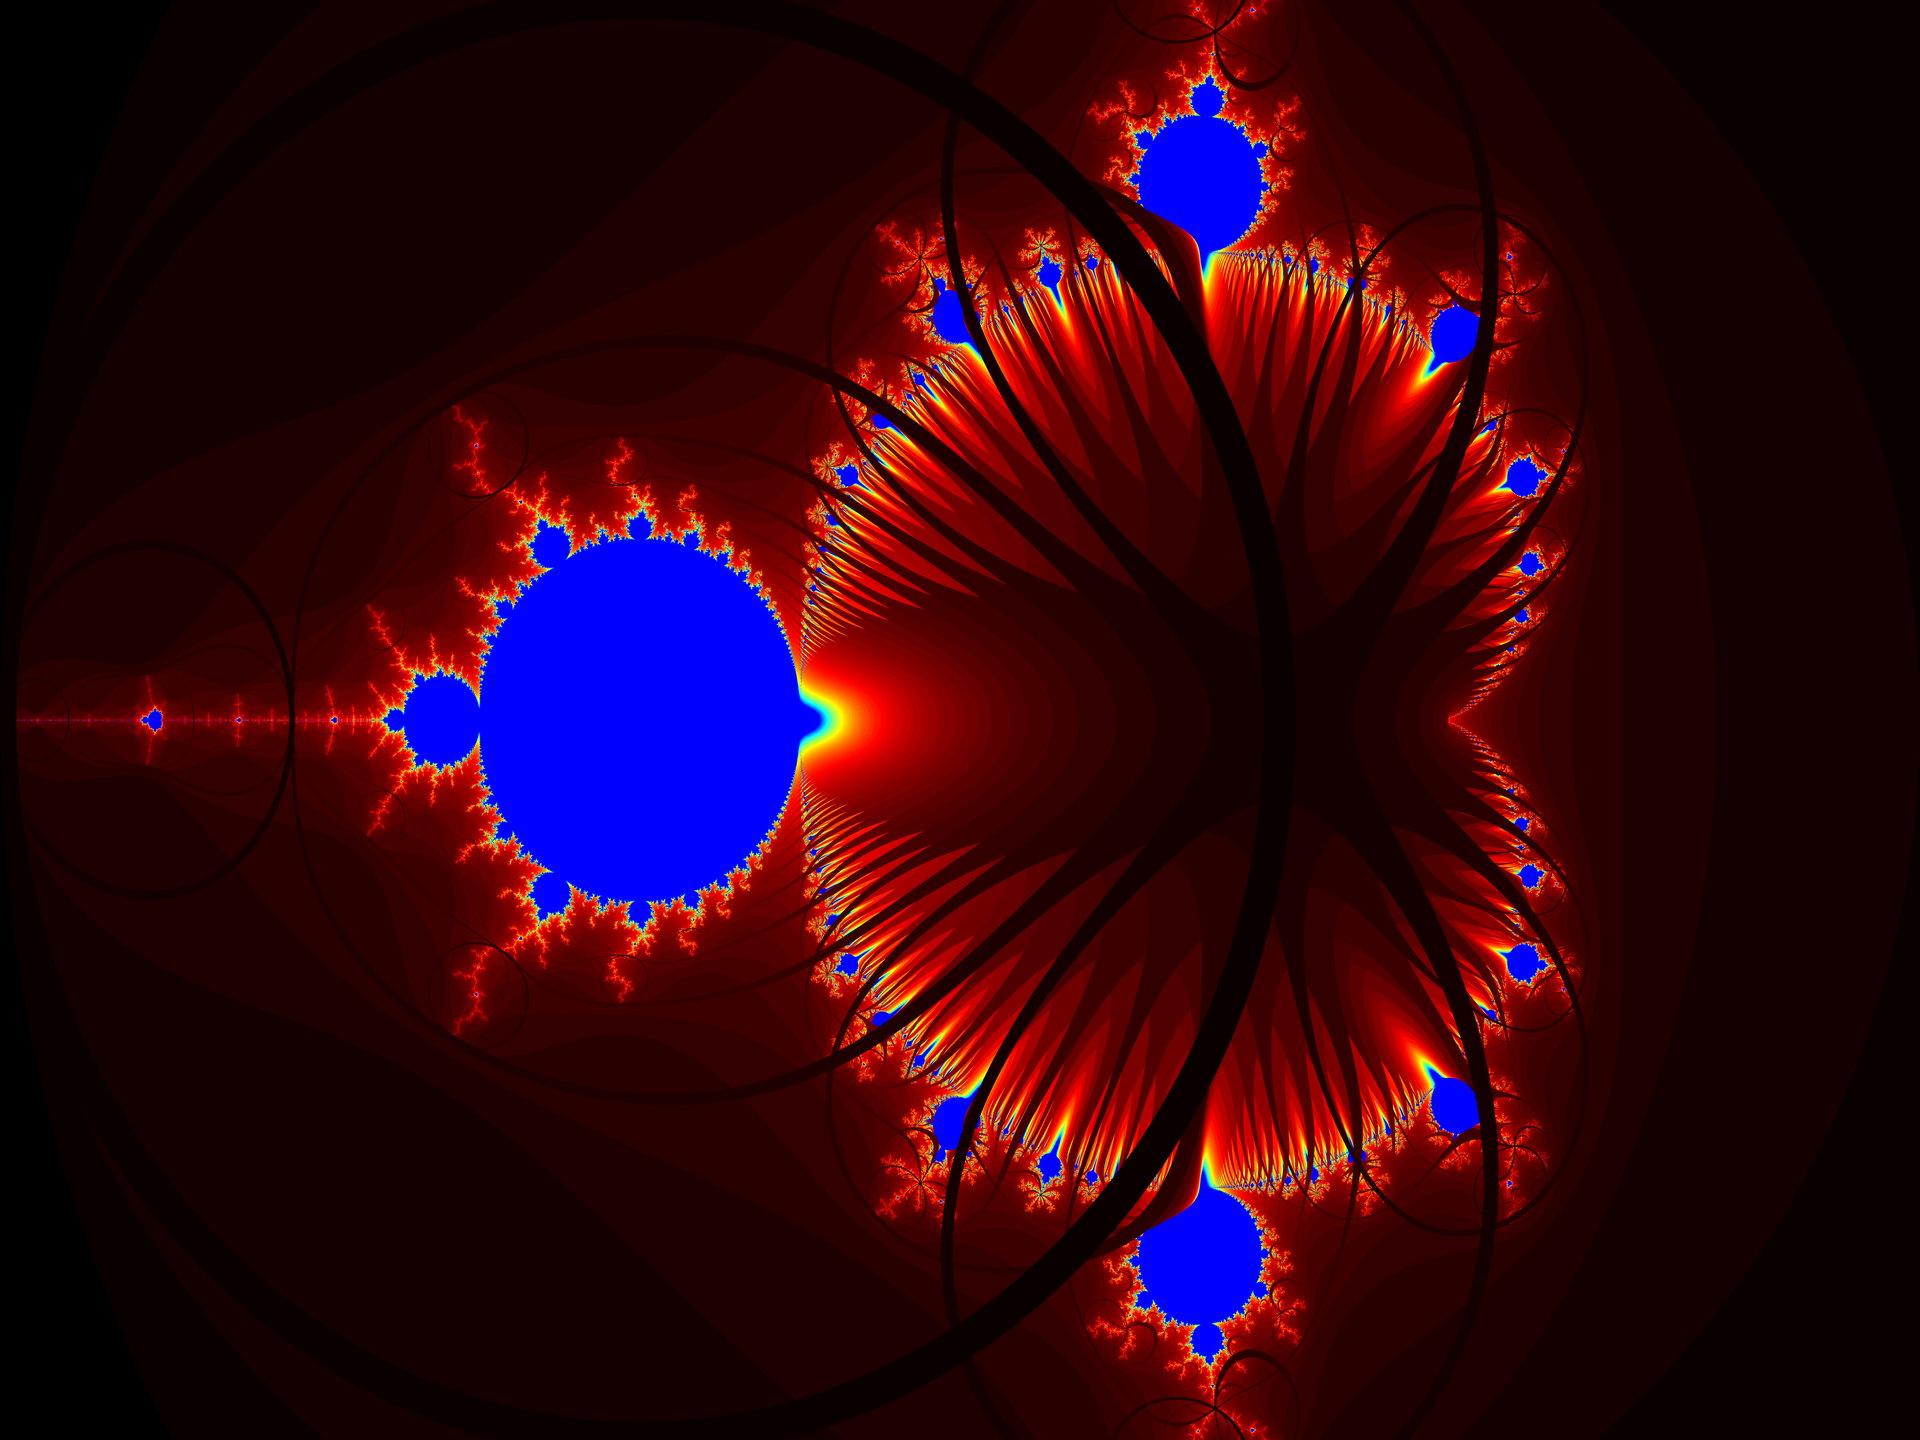
\includegraphics[width=0.7\textwidth]{figures/comparacao/mandelbrot_float.png}
    \caption{Imagem gerada com ponto flutuante.}
    \label{fig:comparison_float}
\end{figure}

Como resultado, a abordagem de encontrar pontos fixos foi descartada para preservar a qualidade das imagens geradas.
\subsection{Paralelismo}

A paralelização é feita utilizando múltiplas threads, controladas pelo parâmetro \texttt{--threads}. Cada thread é responsável por calcular uma fatia da imagem, dividida por linhas. O número de threads pode ser ajustado conforme o número de núcleos disponíveis na máquina.

Devido à alta resolução da imagem (\( 15360 \times 8640 \)) e ao elevado número de iterações (\( 10.000 \)), o tempo de execução ainda pode ser significativo, mesmo com paralelismo. Isso ocorre porque o cálculo de cada ponto no conjunto de Mandelbrot é computacionalmente intensivo, especialmente nas regiões de fronteira, onde a convergência é mais lenta e exige mais iterações para determinar se o ponto pertence ao conjunto. Além disso, a sobrecarga de criação e gerenciamento de threads também contribui para o tempo total de execução.
